%!TEX root = ../thesis.tex

\thispagestyle{myheadings}

\chapter{Straw measurement angular correction}
\label{app:angularcorrection}


The tracker straws don't measure U and V coordinates directly, but instead measure the DCA radii deriving from measured hit times. In order to utilize the minimization procedure described in \secref{sec:TrackFittingAlgorithm} on measured track parameters these radii must first be converted to U and V parameters, and similarly for the U and V errors. To first order the measured DCAs can be used identically as the U and V positions, but it was found that there were slight biases in the truth pulls due to this.

In order to improve the results, angular corrections were made to the DCAs to give more accurate estimates of the ``measured'' positions. It was found that for the error correction, assuming a straight particle path was sufficient for ideal results. For the position correction, it was found that assuming a circular particle path (constant field) correction for the curved tracks was sufficient. These corrections are dependent on the angle of the track, so it's imporant to note that during each successive iteration of the track fitting, the ``measured'' parameters are adjusted by the latest ``predicted'' momenta which change the angle of the track. The correction depends on whether the track went to the left or right side of the wire. Note that the momentum perpendicular to the straw measurement axis can be ignored since it doesn't affect the U or V value. A summary of the calculation of the right side correction follows, with the left side correction being calculated in a similar manner. See Figure \ref{fig:angularCorrection}. 

\begin{figure}[]
	\centering
	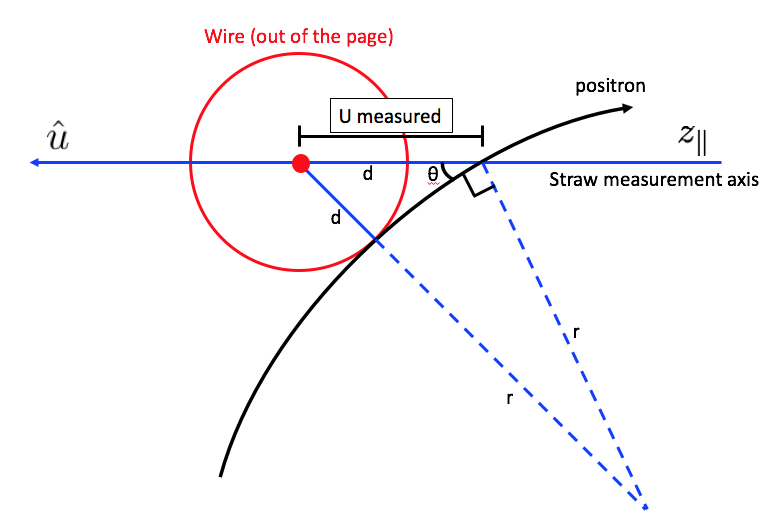
\includegraphics[width=1.0\textwidth]{angularCorrection}
	\caption[Angular correction for measured DCAs]{A positron passing through a straw will produce a hit of radius $d$. The desired value is the U or V position along the straw measurement axis. The positron trajectory can be approximated as a circle in a constant magnetic field over the length of the path across the straw. The curvature for the high energy positrons is small such that $r \gg d$ and the angle between the trajectory and the center of the circle can be approximated as 90\textdegree{}. Sizes and angles are exaggerated. A similar diagram can be drawn for positrons passing to the left of the wire. \textbf{Might want to clean up this picture at some point.}}
	\label{fig:angularCorrection}
\end{figure}

To solve for the measured U (or V) value, first use the following trigonometric identity:
	\begin{align}
		(r+d)^{2} = r^{2}+u^{2}-2ru\cos(90+\theta),
	\end{align}
where $u$ is the parameter of interest. The angle $\theta$ can be determined from 
	\begin{align}
		\hat{z_{\parallel}} \cdot \hat{p_{\parallel}} = \cos{\theta}, \hspace{.1cm} \theta = \cos^{-1}{\frac{p_{\parallel}}{p}}, 
	\end{align}
where $p_{\parallel}$ is the positron momentum anti-parallel to the U measurement axis at the wire plane. Using some further trigonometric identities and solving for u gives
	\begin{align}
		u = -r\sqrt{1-\Big(\frac{p_{\parallel}}{p}\Big)^{2}} + \sqrt{d^{2} + 2dr + r^{2}\Big(1-\Big(\frac{p_{\parallel}}{p}\Big)^{2}\Big)},
	\end{align}
for the right side correction. Similarly,  
	\begin{align}
		u = +r\sqrt{1-\Big(\frac{p_{\parallel}}{p}\Big)^{2}} - \sqrt{d^{2} + 2dr + r^{2}\Big(1-\Big(\frac{p_{\parallel}}{p}\Big)^{2}\Big)},
	\end{align}
for the left side correction. The radius $r$ can be calculated from the momentum and magnetic field at the predicted hit position, and the momentum components can be determined within the Geant4 simulation. The straightline correction to the errors is done simpler manner using the Pythagorean theorem, 
	\begin{align}
		\sigma_{uv}' = \frac{\sigma_{uv}}{\sqrt{1-\big(\frac{p_{\parallel}}{p}\big)^{2}}},
	\end{align}
where $\sigma_{uv}'$ is the improved error from original U or V error $\sigma_{uv}$ on the DCA.
